Les observations des amas de galaxies du grand programme SZ de NIKA2 ont commencé en 2017, avec l'observation de l'amas PSZ2-G144.83+25.11.
Cet amas a bénéficié d'un long temps d'observation dans le cadre de la phase de vérification scientifique de NIKA2.
Par conséquent, les cartes de cet amas offrent une détection hautement significative de l'effet SZ, jusqu'à $13\sigma$.
Cette grande qualité de données a permis une analyse certes profonde et détaillée des propriétés thermodynamiques du milieu intra-amas \cite{ruppin_first_2018}, mais qui n'est pas représentative des observations standard du LPSZ.

Ce chapitre présente la deuxième analyse individuelle d'un amas de galaxies dans le LPSZ.
Cette analyse présente plusieurs intérêts.
D'une part, elle constitue la première analyse de données de qualité standard pour le LPSZ.
D'autre part, elle se focalise sur \act, un amas distant et de faible masse, ayant pour conséquence un signal SZ faible et peu étendu.
Les cartes NIKA2 de cet amas sont de plus fortement contaminées par des sources ponctuelles, dont le flux compense une proportion non négligeable du signal SZ de l'amas (comme nous le verrons en page \pageref{sec:act:ps}).
Cet amas représente donc un banc d'essai pour les analyses des sources les plus complexes du grand programme SZ.
Cette analyse et ses résultats sont publiés dans \myfullcite{keruzore_exploiting_2020}.

% ==================================================================================== %
\section{Observations de ACT-CL J0215.4+0030}

% ------------------------------------------------------------------------------------ %
\subsection{Détection de l'amas par l'Atacama Cosmology Telescope}\label{subsec:act:act}

L'amas \act\ a été découvert par le premier relevé SZ de l'Atacama Cosmology Telescope (ACT), à un redshift de 0.865 \cite{menanteau_atacama_2013,hasselfield_atacama_2013}.
Il y a été détecté avec une signifiance de $5.5\sigma$.
Faute d'avoir une résolution angulaire suffisante pour résoudre des amas distants, le catalogue ACT reporte pour cet amas uniquement une mesure de signal SZ intégré, $Y_{500}$.
La masse de cet amas, estimée grâce à la relation d'échelle $Y_{500} - M_{500}$ publiée par \myciteauthor{arnaud_universal_2010}, est de $M_{500} = 3.8 \times 10^{14} \; M_\odot$.

% ------------------------------------------------------------------------------------ %
\subsection{Observations de l'amas avec NIKA2}\label{subsec:act:nk2}

Les observations NIKA2 de \act\ ont eu lieu lors de la quatorzième campagne d'observations de NIKA2.
Elles sont réparties sur cinq jours, entre le 17 et le 22 janvier 2018.
Toutes les observations de l'amas ont été effectuées entre 16h et 22h15 (UT).
La focalisation du télescope a été vérifiée au début de chaque série d'observations.
Le pointage du télescope et le lobe de NIKA2 ont quant à eux été vérifiés toutes les heures au cours des observations.
L'amas a été observé 8.6 heures au total, dans des conditions stables, avec une opacité moyenne à 225 GHz de $\tau_{225} = 0.175 \pm 0.05$.
Les distributions de l'opacité et de la transmission atmosphérique au cours des observations sont représentés sur la figure \ref{fig:act:scans}, montrant une grande proportion d'observations réalisées dans de mauvaises conditions (à des élévations inférieures à 30\textdegree, ou à des transmissions atmosphériques inférieures à 0.75).
Puisque les objectifs de rapport signal sur bruit du LPSZ demandaient 9 heures d'observations avec une opacité\footnote{correspondant à une transmission atmosphérique supérieure à 0.8, voir section \mypageref{sec:30m_geo}.} de $\tau_{225} = 0.1$, un bruit plus élevé que l'objectif est attendu dans les cartes NIKA2.

\begin{figure*}[t]
    \centering
    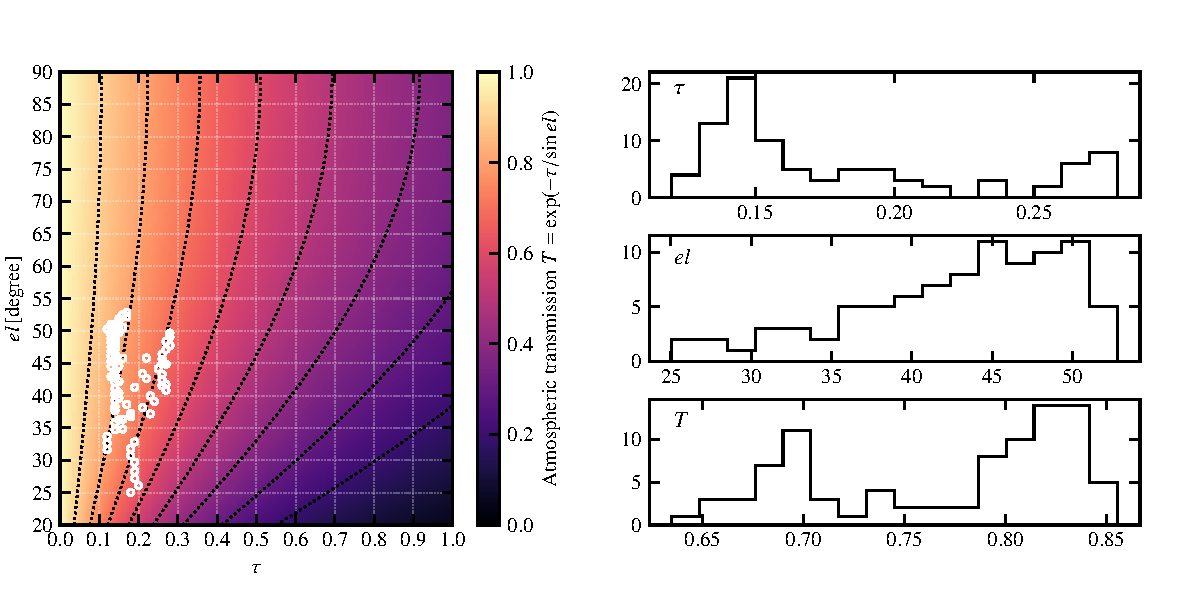
\includegraphics[width=\linewidth]{Figures/Chap_actj0215/scans.pdf}
    \caption{
        \textit{Gauche}: transmission atmosphérique $T$ en fonction de l'opacité $\tau$ et de l'élévation $el$.
        Chaque point blanc représente un scan de \act.
        \textit{Droite}: Distribution des opacités (\textit{haut}), élévations (\textit{centre}), et transmissions atmosphériques (\textit{bas}) pour les scans de \act.
    }
    \label{fig:act:scans}
\end{figure*}

Les observations ont été réalisées sous forme de plusieurs séries de quatre scans OTF, décrits en section \ref{sec:nk_otf_toi} de 8' $\times$ 4', chacun composé de 25 \textit{subscans}, avec des angles de 0, 45, 90 et 135 degrés par rapport à l'axe des ascensions droites.
Le centre de ces scans a été choisi aux coordonnées de l'amas reportées par le catalogue ACT \cite{menanteau_atacama_2013}, c'est-à-dire (RA, Dec)$_{\rm J2000}$ = (02h 15m 28.8s +00\textdegree 30' 33.0'')

Le pipeline de la collaboration NIKA2 décrit dans le chapitre \ref{chap:decorr} a été utilisé pour le traitement des données brutes de NIKA2.
La décorrélation du signal astrophysique et des différentes sources de bruit a été réalisée en utilisant la méthode \textit{Common mode one block}, décrite dans le chapitre \ref{chap:decorr}, ainsi que dans \myciteauthor{perotto_calibration_2020} sous le nom de \textit{most correlated pixels}.
Le masque utilisé pour le calcul du mode commun a été défini comme un disque de diamètre 2'  au centre de la carte.
Les itérations sur le masque basées sur des niveaux de signal sur bruit n'ont montré aucune amélioration des cartes, soustrayant au fur et à mesure des itérations plus de signal sans diminuer le niveau de bruit.
Par conséquent, la carte obtenue avec un masque circulaire a été retenue pour le reste de l'analyse.

La fonction de transfert, quantifiant le filtrage dû à la soustraction du bruit, ainsi que le spectre de puissance du bruit résiduel, sont produits automatiquement par le logiciel de réduction des données brutes utilisant le pipeline de la collaboration NIKA2 (cf. section \ref{sec:perf_decor}).
Ils sont tous deux présentés dans la figure \ref{fig:act:tf_noise}.
Il y apparaît que le signal est bien préservé aux petites échelles angulaires ($k > 0.5 \; {\rm arcmin}^{-1}$), et que le bruit résiduel est fortement corrélé.

\begin{figure}
    \centering
    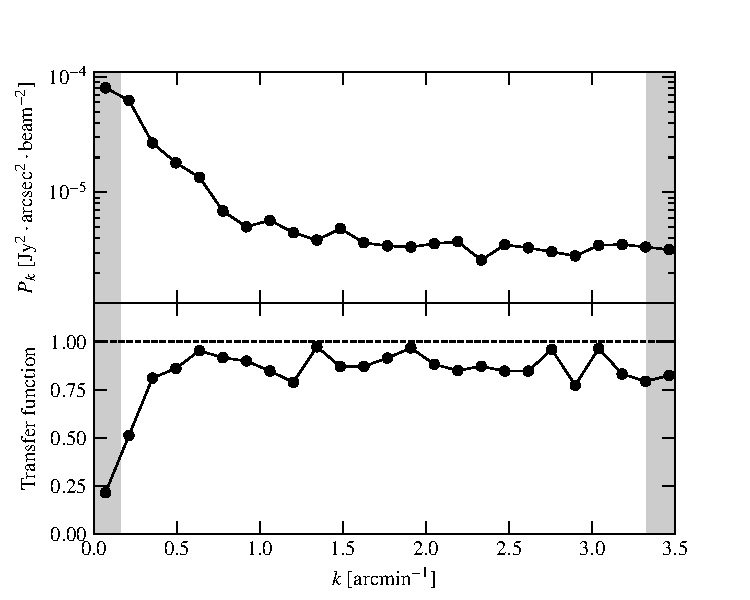
\includegraphics[height=8cm, trim={0cm, 0cm, 0cm, 1cm}, clip]{Figures/Chap_actj0215/TF_noise.pdf}
    \caption{
        Spectre de puissance du bruit résiduel (\textit{haut}) et fonction de transfert (\textit{bas}) correspondant à l'analyse des observations de \act\ avec NIKA2
        La procédure d'obtention est décrite dans \ref{sec:perf_decor}.
        Le spectre de puissance montre un bruit résiduel corrélé à grande échelle, et la fonction de transfert montre le filtrage du signal aux grandes échelles angulaires.
    }
    \label{fig:act:tf_noise}
\end{figure}

Les cartes NIKA2 utilisées pour l'analyse sont présentées dans la figure \ref{fig:act:nkmaps}.
Dans la partie gauche, correspondant à la carte NIKA2 à 150 GHz, l'amas peut être identifié comme un décrément au centre de la carte, caractéristique de l'effet tSZ à des fréquences inférieures à 217 GHz.
Le maximum de ce décrément est détecté avec un rapport signal sur bruit de $8.5\sigma$.
On remarque dans cette carte un haut niveau de bruit résiduel, se manifestant par un gradient dans le sens sud ouest -- nord est.

La carte NIKA2 à 150 GHz montre également une indication de contamination par des sources ponctuelles.
Celles-ci émettent un flux positif qui peut compenser le décrément de l'effet SZ, et créer des trous\footnotemark\ dans la forme apparente du milieu intra-amas.
Une telle contamination est particulièrement inquiétante dans le cas de cet amas.
En effet, étant donné son faible signal (moins d'un mJy/beam au maximum) et sa petite extension spatiale (environ dix fois l'angle solide du lobe de NIKA2), la moindre contamination peut avoir de grandes conséquences sur les propriétés physiques reconstruites.

Dans la partie droite de la figure \ref{fig:act:nkmaps}, correspondant à la carte NIKA2 à 260 GHz, aucun signal SZ n'est détecté.
Le signal SZ positif attendu à ces fréquences ($\sim 0.2$ mJy/beam) est inférieur au niveau de bruit au centre de la carte par un facteur quatre.
En revanche, cette carte nous permet de confirmer la présence de sources ponctuelles proches du centre de l'amas, correspondant aux positions auxquelles des trous sont observés dans le signal SZ de l'amas.
Cela indique qu'une prise en compte soigneuse de la contamination par ces sources sera nécessaire à la mesure des propriétés thermodynamiques du milieu intra-amas.

\begin{figure}[t]
    \centering
    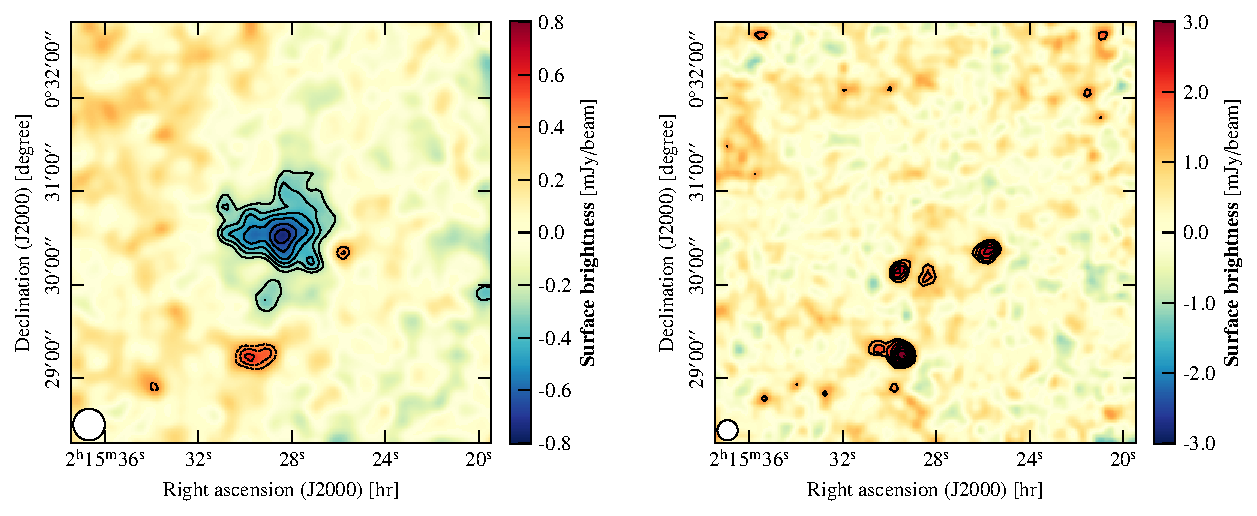
\includegraphics[width=\textwidth]{Figures/Chap_actj0215/nk_maps.pdf}
    \caption{
        Cartes NIKA2 du champ de l'amas à 150~GHz (\textit{gauche}) et 260~GHz (\textit{droite}).
        Chaque carte est montrée dans un champ carré de 4.5' $\times$4.5'  centré sur les coordonnées observées.
        Dans chacune des cartes, les contours noirs montrent les niveaux de signal sur bruit commençant à $3\sigma$ et espacés de $1\sigma$.
        Les cartes de gauche et droite sont lissées avec un noyau Gaussien de 10''  et 6''  respectivement pour des raisons visuelles.
        Pour chaque carte, la FWHM de sa résolution effective est illustrée par un disque blanc en bas de la carte.
    }
    \label{fig:act:nkmaps}
\end{figure}

% ------------------------------------------------------------------------------------ %
\subsection{Observations de l'amas avec \textit{XMM-Newton}}\label{subsec:act:xmm}

\act\ a été observé par \textit{XMM-Newton} pendant 37 ks.
Les données ont été récupérées depuis l'archive XMM, et les procédures standard (voir, par exemple, \cite{bartalucci_resolving_2017}) ont été suivies pour produire des fichiers étalonnés répertoriant les évènements enregistrés.
Les données ont été corrigées des effets de vignettage et du signal de fond.
Les sources ponctuelles ont été détectées et exclues.
Après ce nettoyage, le temps d'observation était de 35 ks sur les caméras MOS, et de 29 ks sur la caméra pn.

La carte lissée par ondelettes montrée sur la figure~\ref{fig:act:xmm} montre que le milieu intra-amas semble perturbé.
Les profils de densité et température électroniques corrigées de la PSF ont été produits à partir des données de \textit{XMM-Newton} en utilisant la déprojection décrite dans \cite{pratt_gas_2010}.
Au vu de la nature possiblement perturbée de l'amas, ces profils extraits aux pics X et SZ ont été comparés, mais aucune différence significative n'a été détectée.
Les profils 3D extraits au pic SZ sont montrés dans la partie droite de la figure \ref{fig:act:xmm}.
Le profil de température projeté, extrait directement à partir des spectres 2D, est aussi montré pour référence, mais seul le profil 3D est utilisé dans le reste de l'analyse.

\begin{figure}[t]
    \centering
    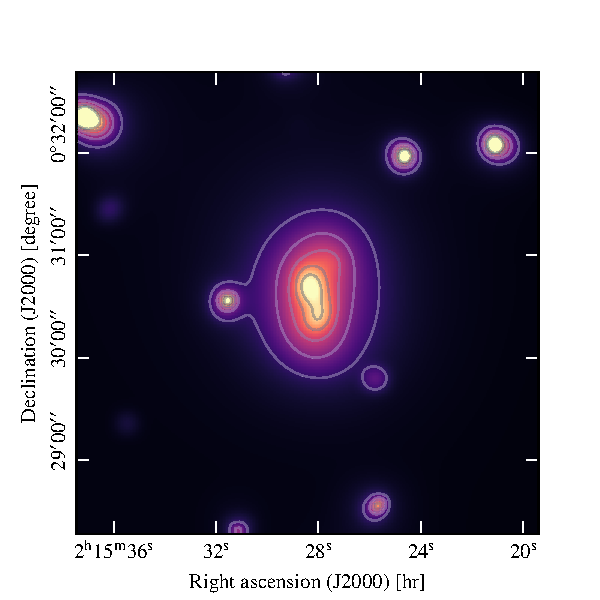
\includegraphics[height=7cm, trim={0cm, 0cm, 1cm, 1cm}, clip]{Figures/Chap_actj0215/xmm_map.pdf}
    \hfill
    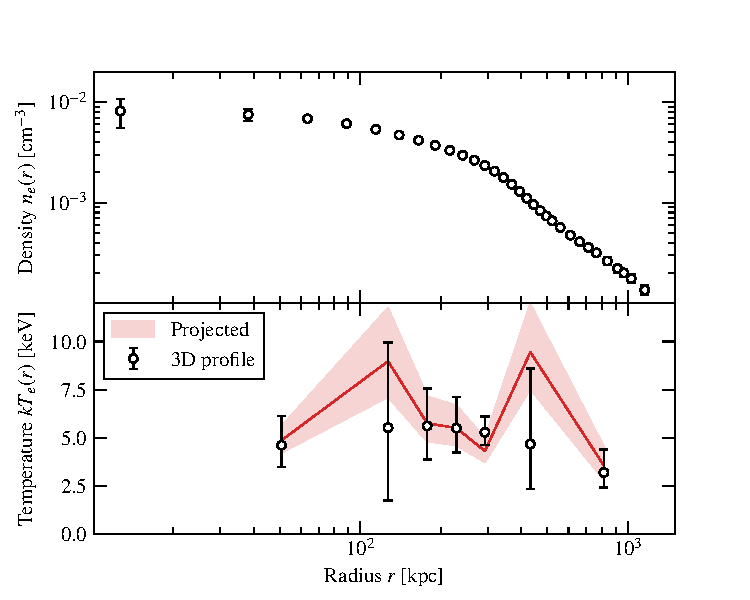
\includegraphics[height=7cm, trim={0cm, 0cm, 1cm, 1cm}, clip]{Figures/Chap_actj0215/xmm_profs.pdf}
    \caption[XMM]{%
        \textbf{Gauche:} Carte d'évènements \textit{XMM-Newton} lissée par ondelettes.
        La région montrée est la même que dans la figure~\ref{fig:act:nkmaps}.
        Les iso-contours sont montrés en gris.
        \textbf{Droite:} Profils de densité (\textit{haut}) et température (\textit{bas}) électronique extraits à partir des observations XMM de l'amas.
        Les profils sont extraits aux coordonnées du pic SZ, comme décrit dans le texte (\ref{subsec:act:xmm}).
        Les barres d'erreur montrent les incertitudes à $1\sigma$.
        Pour le profil de température, la ligne rouge représente le profil projeté,tandis que les points blancs représentent le profil 3D reconstruit ; pour une explication détaillée de la différence entre les deux quantités, voir \cite{pratt_gas_2010}.
    }
    \label{fig:act:xmm}
\end{figure}

% ==================================================================================== %
\section{Contamination par des sources ponctuelles}\label{sec:act:ps}

Comme nous l'avons vu précédemment, une estimation précise de la contamination par des sources ponctuelles est nécessaire dans l'objectif de mesurer les propriétés du milieu intra-amas.
Cette étude est cruciale dans le cas de cet amas, étant donné son faible signal et sa faible extension spatiale.
Dans cette section, nous présentons la méthodologie utilisée pour estimer l'amplitude de cette contamination.

% ------------------------------------------------------------------------------------ %
\subsection{Identification des sources ponctuelles}

Dans le cas de \act, quatre sources sont identifiées avec un rapport signal sur bruit supérieur à 3 dans la carte NIKA2 à 260 GHz.
Leurs flux sont plus élevés à 260 GHz qu'à 150 GHz, favorisant l'hypothèse de sources sub-milimétriques (SMG) plutôt que radio.
Cette hypothèse est confirmée par l'identification de ces sources dans le catalogue HerS82 \cite{viero_herschel_2014}, construit grâce à l'instrument SPIRE à bord du satellite \textit{Herschel} qui a observé le ciel dans le domaine sub-millimétrique.
Ce catalogue nous permet également d'identifier une cinquième source dans le nord-est de l'amas.

La figure \ref{fig:act:composite} montre une carte composite multifréquence de la région de l'amas.
Les cercles verts sont centrés sur les positions des cinq SMG itentifiées dans le catalogue HerS82, et le diamètre de chaque cercle correspond à la FWHM du lobe instrumental de SPIRE à 250 $\mu$m, bande à laquelle la résolution angulaire de SPIRE est la meilleure.
Les régions rouges représentent les niveaux de rapport signal sur bruit dans la carte NIKA2 à 260 GHz lorsque celui-ci est supérieur à $3\sigma$.
NIKA2 et SPIRE sont en accord pour les positions des trois sources les plus proches de l'amas: de gauche à droite, SMG1, SMG2, et SMG4.
Dans le nord-est de l'amas, on trouve SMG3, qui est identifiée dans le catalogue HerS82 mais a un signal sur bruit inférieur à $3\sigma$ dans NIKA2 à 260 GHz.
Dans le sud de l'amas, deux sources semblent être résolues par NIKA2, mais seulement la plus faible des deux (S5) est identifiée dans le catalogue HerS82.
Il est par conséquent difficile d'estimer l'amplitude de leur contamination du signal SZ, puisqu'il n'existe pas de moyen de déterminer si le flux de S5 dans les bandes SPIRE provient d'une seule source ou de la somme des deux détectées dans NIKA2.
Ces sources étant jugées suffisamment éloignées de l'amas et de la zone dans laquelle le signal SZ est significatif, elles sont soustraites de la carte NIKA2 à 150 GHz dans la suite de l'analyse.

\begin{figure}[t]
    \centering
    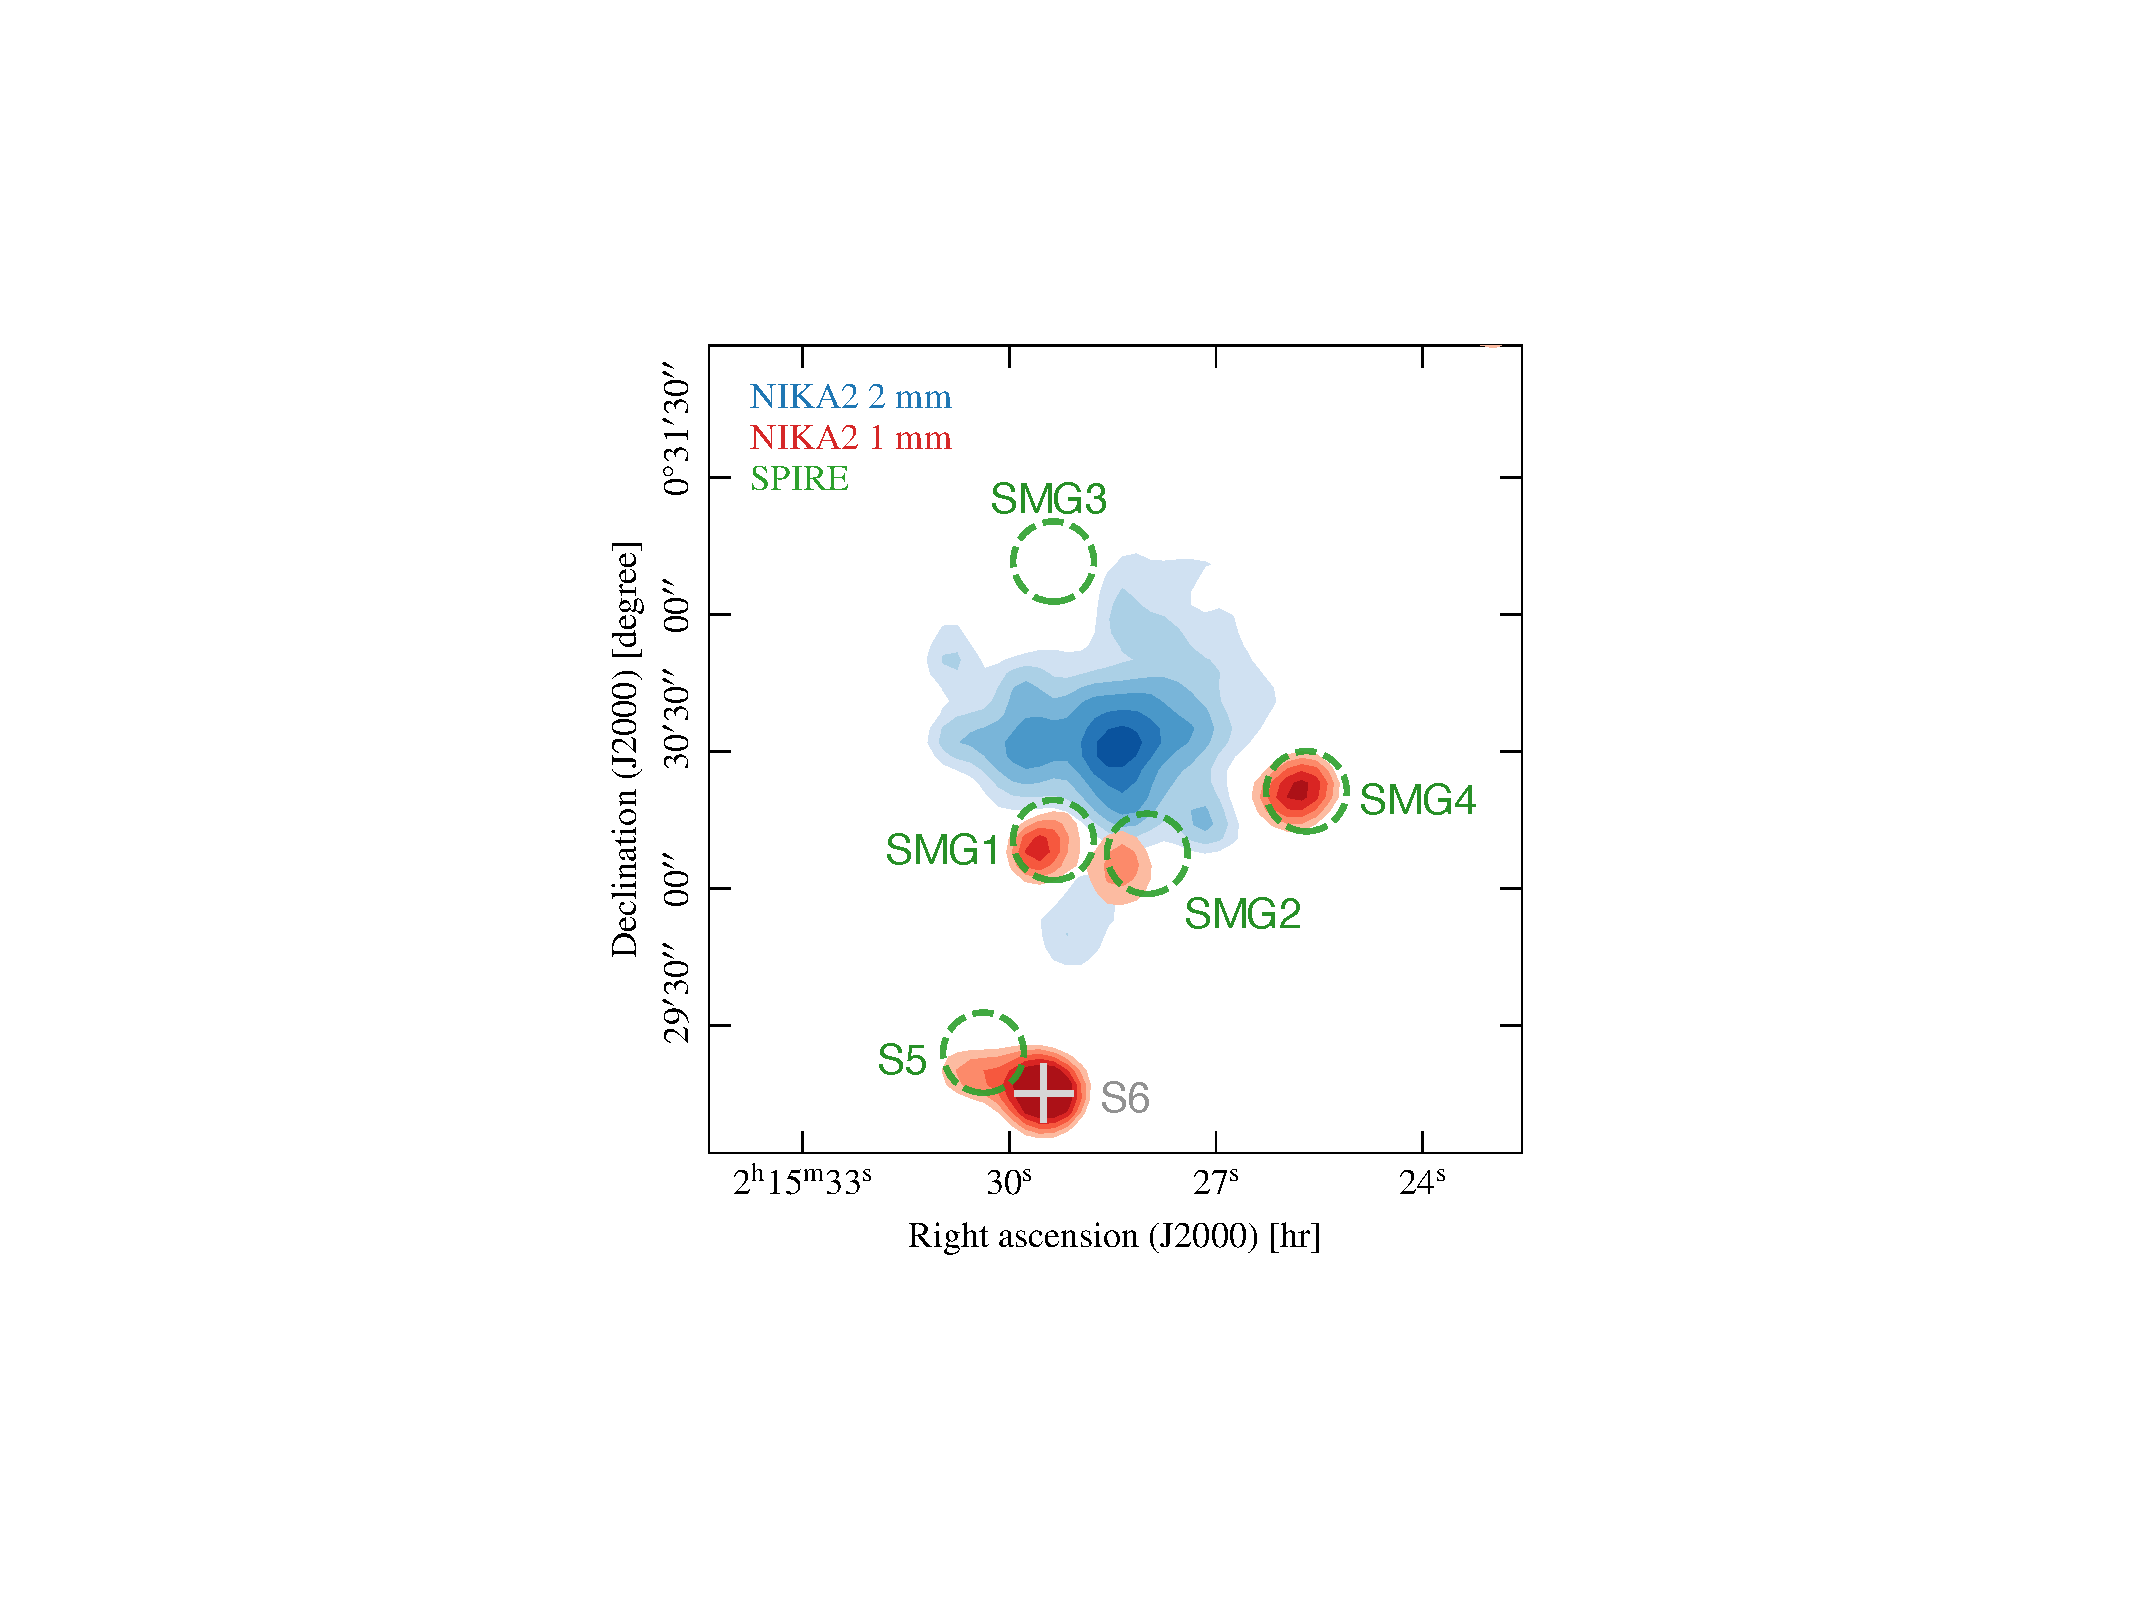
\includegraphics[height=8.5cm, trim={10cm 5cm 8cm 5cm}, clip]{Figures/Chap_actj0215/composite.pdf}
    \caption{%
        Carte composite multifréquence de la région de l'amas.
        Les niveaux de bleu correspondent aux niveaux de signal sur bruit du décrément SZ dans la carte NIKA2 à 150 GHz, commençant à $3\sigma$ et espacés de $1\sigma$.
        De même, les niveaux de rouge correspondent au signal sur bruit des sources ponctuelles dans la carte NIKA2 à 260 GHz.
        Les cercles verts sont centrés sur les positions des sources dans le catalogue HerS82 \cite{viero_herschel_2014} et leur diamètre est la FWHM du lobe instrumental de SPIRE à 250 $\mu$m.
        La croix grise marque la position de S6, la source identifiée par NIKA2 qui n'a pas de contrepartie dans le catalogue HerS82.
        }
    \label{fig:act:composite}
\end{figure}

% ------------------------------------------------------------------------------------ %
\subsection{Estimation de la contamination}\label{subsec:act:sed}

Il est important de noter dans cette analyse l'absence d'information sur l'émission des sources à des fréquences supérieures à celles des bandes passantes de SPIRE ; par exemple, les études précédentes d'observations d'amas avec NIKA et NIKA2 tiraient parti de l'existence de données publiques de l'instrument PACS \cite{poglitsch_photodetector_2010}, qui ne sont pas disponibles ici.
Nous utilisons le logiciel \texttt{PSTools}, présenté en section \mypageref{sec:decor:pstools}, pour estimer l'amplitude de la contamination.
Le flux de chacune des sources est mesuré dans la carte NIKA2 à 260 GHz en ajustant un modèle de lobe instrumental de largeur fixe FWHM=12.5'', d'amplitude et de position libre, dans une portion carrée de largeur 1' autour de la position de la source dans le catalogue HerS82.
Les sources SMG1 et SMG2 étant proches, elles sont ajustées simultanément afin d'éviter une surestimation de leurs flux respectifs.
La SED de chaque source est ensuite ajustée par MCMC sur les points SPIRE et NIKA2 à 260 GHz, en considérant le modèle de corps noir modifié donné par l'équation (\ref{eq:pstools:sed}) et les \prior\ sur les paramètres présentés en \ref{sec:decor:pstools}.
Les échantillons dans l'espace des paramètres sont ensuite utilisés pour calculer une SED qui est extrapolée dans la bande passante de NIKA2 à 150 GHz, ce qui donne une estimation de la densité de probabilité de l'amplitude de la contamination.

La SED ajustée et la distribution de probabilité du flux à 150 GHz de chaque source sont présentés en figure \ref{fig:act:sed}.
On voit que l'ajustement de SED est correct pour toutes les sources, avec des modèles passant bien par les points.
On remarque également que la distribution de probabilité du flux de chaque source à 150 GHz n'est pas gaussienne, et apparaît asymétrique.
La capacité de \texttt{PSTools} à fournir ces distributions comme produit de sortie permettra de les utiliser comme \prior\ sur les flux des sources dans notre analyse, plutôt que de supposer une distribution gaussienne avec une valeur moyenne et une dispersion.

\begin{figure*}[p]
    \centering
    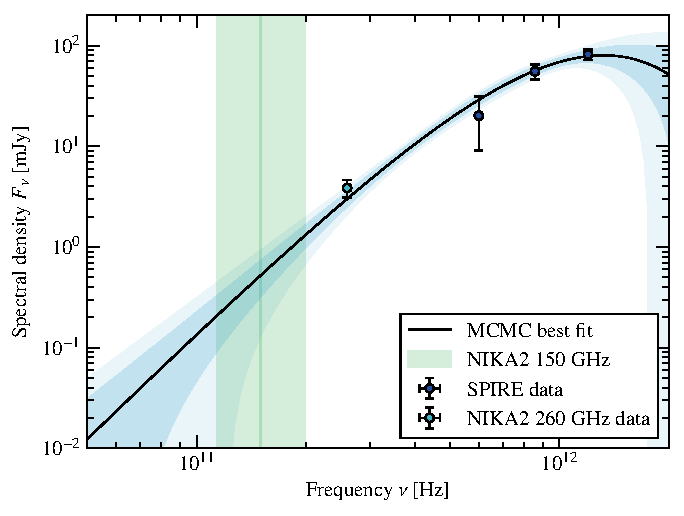
\includegraphics[height=0.23\textheight]{Figures/Chap_actj0215/PSPlots/1_SED_no2mm.pdf} \hspace{20pt}
    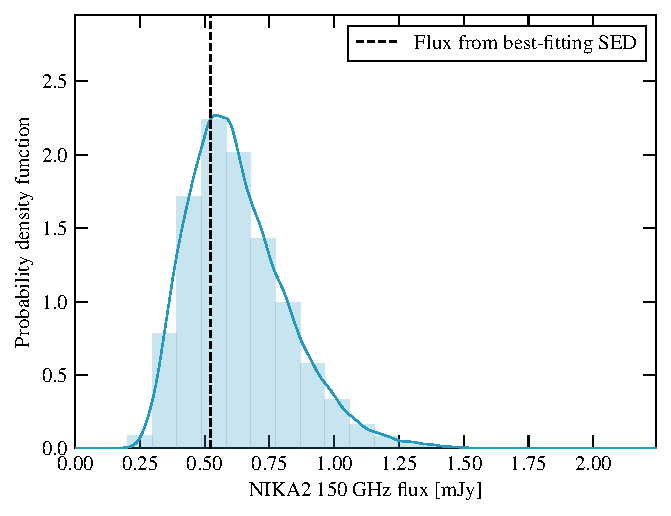
\includegraphics[height=0.23\textheight]{Figures/Chap_actj0215/PSPlots/1_2mm_flux_dist.pdf}
    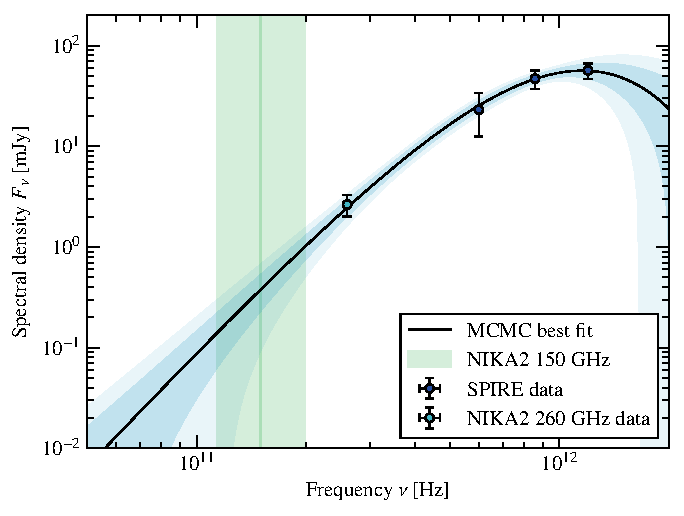
\includegraphics[height=0.23\textheight]{Figures/Chap_actj0215/PSPlots/2_SED_no2mm.pdf} \hspace{20pt}
    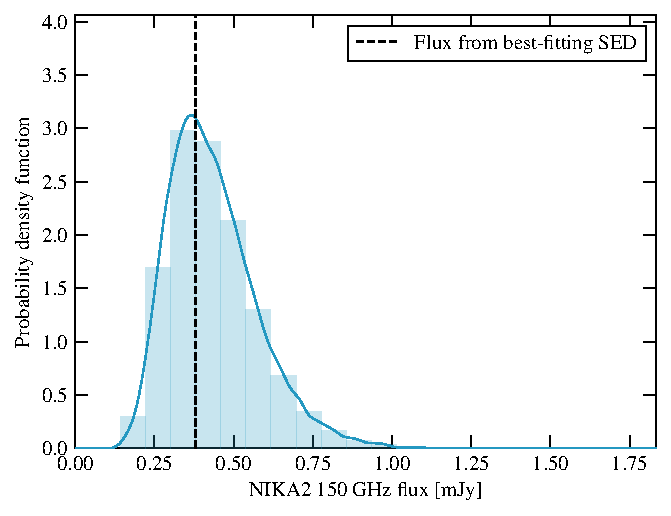
\includegraphics[height=0.23\textheight]{Figures/Chap_actj0215/PSPlots/2_2mm_flux_dist.pdf}
    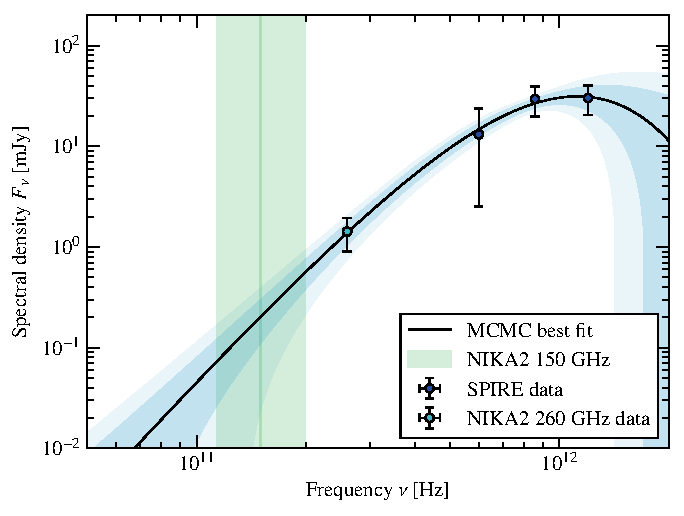
\includegraphics[height=0.23\textheight]{Figures/Chap_actj0215/PSPlots/3_SED_no2mm.pdf} \hspace{20pt}
    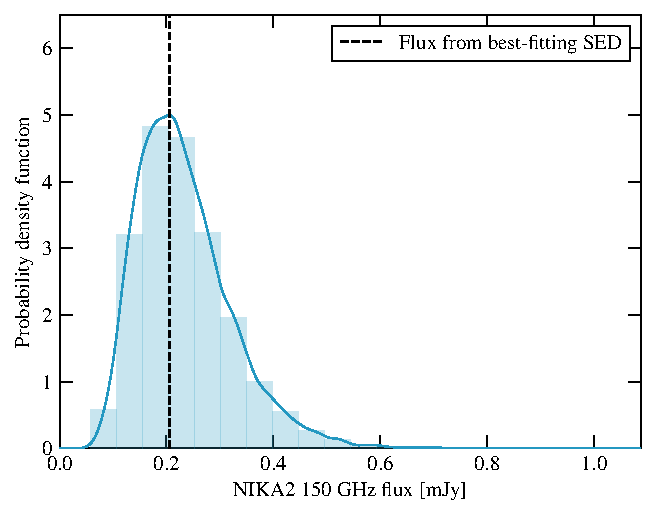
\includegraphics[height=0.23\textheight]{Figures/Chap_actj0215/PSPlots/3_2mm_flux_dist.pdf}
    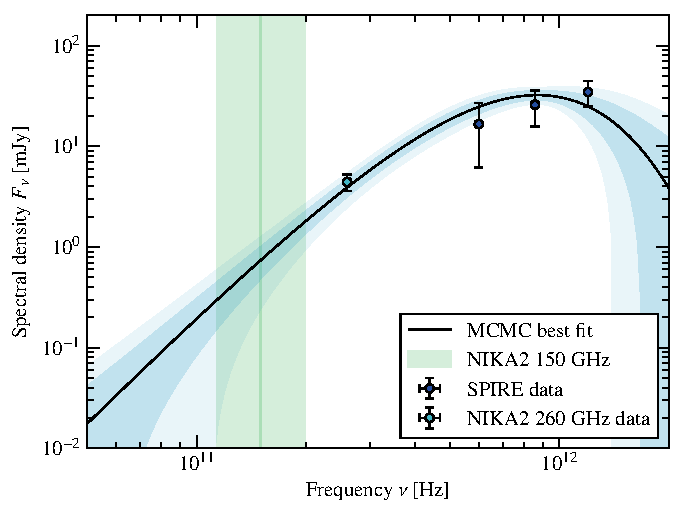
\includegraphics[height=0.23\textheight]{Figures/Chap_actj0215/PSPlots/4_SED_no2mm.pdf} \hspace{20pt}
    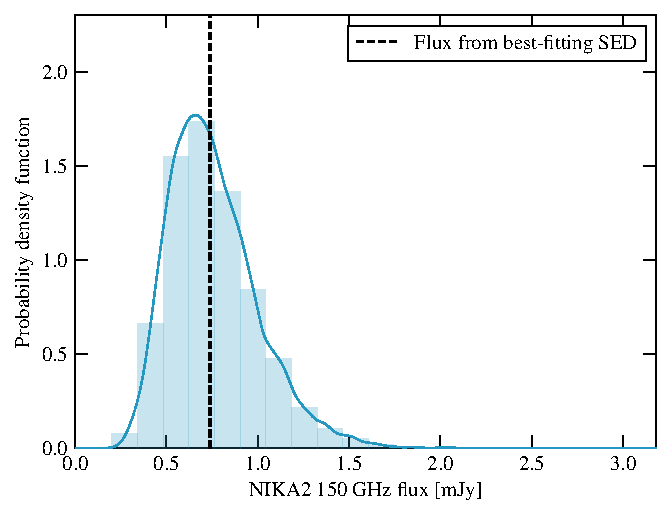
\includegraphics[height=0.23\textheight]{Figures/Chap_actj0215/PSPlots/4_2mm_flux_dist.pdf}
    \caption{
        De haut en bas, résultats de \texttt{PSTools} pour les sources SMG1 à SMG4 dans le champ de l'amas \act.
        \textbf{Gauche:} ajustement de la SED sur les flux SPIRE (bleu foncé) et NIKA2 à 260 GHz (bleu clair).
        La région verte correspond à la bande passante de NIKA2 à 150 GHz.
        Les régions bleues correspondent aux intervalles de confiance à 1$\sigma$ et 2$\sigma$ sur l'ajustement de la SED.
        \textbf{Droite:} distribution de probabilité du flux à 150 GHz.
        L'histogramme représente les flux obtenus pour les chaînes de Markov, et la courbe bleue est la distribution de probabilité résultante.
    }
    \label{fig:act:sed}
\end{figure*}

% ------------------------------------------------------------------------------------ %
\subsection{Résultats}

La table \ref{tab:act:pscat} présente les flux et positions des six sources considérées dans cette analyse.
La dernière colonne présente le flux attendu dans la carte NIKA2 à 150 GHz de chaque source, obtenu par ajustement puis extrapolation de SED.
Il est important de noter que ces flux peuvent atteindre jusqu'à 0.74 mJy, alors que le pic d'émission SZ de l'amas est inférieur à 0.8 mJy/beam.
Cela accentue l'importance de la prise en compte de la contamination par les sources ponctuelles dans cette analyse.

L'une des sources (SMG2) présente également une émission radio.
Celle-ci est détectée dans le dernier catalogue FIRST \cite{helfand_last_2015} avec une densité de flux à 1.4 GHz de $2.22 \pm 0.10 \; \mathrm{mJy}$.
L'absence de couverture de la région de l'amas à d'autres fréquences radio rend impossible l'ajustement de la SED de l'émission radio de cette source.
Elle est donc modélisée par une loi de puissance $F(\nu) = F(\nu_0)\times(\nu/\nu_0)^\alpha$ avec un indice spectral $\alpha=-0.7 \pm 0.2$, qui est une bonne approximation de la SED de galaxies émettrices en radio \cite{condon_cosmological_1984}.
L'extrapolation de cette loi de puissance dans la bande passante à 150 GHz de NIKA2 donne une estimation de la densité de flux radio de cette source, $F_\mathrm{radio}(\mathrm{150\; GHz}) = 83 ^{+127}_{-50} \,\mathrm{\mu Jy}$.
Cette contribution est ajoutée à celle calculée par extrapolation de SED dans le domaine sub-millimétrique pour obtenir une estimation de la densité de flux totale de la source, bien que la contribution radio soit négligeable devant l'émission thermique de la poussière.

\begin{table*}[tp]
    \begin{center}
    \footnotesize
    \begin{tabular}{ccccccc}
        \toprule
        Source & Coordonnées J2000 & 1200 GHz & 860 GHz & 600 GHz & 260 GHz & 150 GHz \\
            &  & [mJy] & [mJy] & [mJy] & [mJy] & [mJy] \\
        \midrule
        SMG1 & $02^\mathrm{h}15^\mathrm{m}29.5^\mathrm{s}$ $+00^\circ30{}^\prime07.2{}^{\prime\prime}$ & 81.55 $\pm$ 9.77 & 55.39 $\pm$ 9.63 & 20.14 $\pm$ 11.08 & 3.85 $\pm$ 0.77 & 0.62 $\pm$ 0.19 \\
        SMG2 & $02^\mathrm{h}15^\mathrm{m}28.3^\mathrm{s}$ $+00^\circ30{}^\prime03.5{}^{\prime\prime}$ & 56.57 $\pm$ 9.83 & 46.87 $\pm$ 9.83 & 23.07 $\pm$ 10.57 & 2.64 $\pm$ 0.64 & 0.38 $\pm$ 0.14 $^{(a)}$\\
        SMG3 & $02^\mathrm{h}15^\mathrm{m}29.1^\mathrm{s}$ $+00^\circ31{}^\prime10.2{}^{\prime\prime}$ & 30.19 $\pm$ 9.68 & 29.45 $\pm$ 9.69 & 13.13 $\pm$ 10.6 & 1.42 $\pm$ 0.52 & 0.21 $\pm$ 0.09 \\
        SMG4 & $02^\mathrm{h}15^\mathrm{m}25.7^\mathrm{s}$ $+00^\circ30{}^\prime21.3{}^{\prime\prime}$ & 34.6 $\pm$ 9.86 & 25.84 $\pm$ 10.11 & 16.58 $\pm$ 10.43 & 4.42 $\pm$ 0.83 & 0.74 $\pm$ 0.25 \\
        S5 & $02^\mathrm{h}15^\mathrm{m}30.0^\mathrm{s}$ $+00^\circ29{}^\prime12.6{}^{\prime\prime}$ & -- & -- & -- & -- & 0.66 $\pm$ 0.19 $^{(b)}$\\
        S6 & $02^\mathrm{h}15^\mathrm{m}29.0^\mathrm{s}$ $+00^\circ29{}^\prime14.2{}^{\prime\prime}$ & -- & -- & -- & -- & 0.61 $\pm$ 0.19 $^{(b)}$\\
        \bottomrule\\
    \end{tabular}
    \normalsize
    \end{center}
    \vspace{-10pt}
    \caption{%
        Catalogue des positions et flux des six sources sub-millimétriques détectées dans un rayon de 2.5' autour du centre de \act.
        Les flux à 1200, 860 et 600 GHz proviennent du catalogue HerS82 \cite{viero_herschel_2014}.
        Les coordonnées et flux à 260 GHz sont obtenues par ajustement de modèles de lobe dans la carte NIKA2 à 260 GHz.
        Les flux à 150 GHz et leurs barres d'erreur sont les moyennes et écarts type des distributions de flux dans la bande passante de NIKA2.
        $^{(a)}$ Flux incluant l'émission radio.
        $^{(b)}$ Flux mesurés directement dans la carte NIKA2 à 150 GHz.
    }
    \label{tab:act:pscat}
\end{table*}

Les distributions de probabilité des flux à 150 GHz obtenues seront utilisées dans cette analyse afin de considérer la contamination par les sources ponctuelles comme des paramètres de nuisance lors de l'ajustement du profil de pression de \act.
Cette approche est préférée à une simple soustraction des sources dans le but de propager l'incertitude sur les flux des sources aux mesures des propriétés du milieu intra-amas, en traitant la contamination comme un effet systématique affectant l'analyse.
Cette procédure est décrite dans la section suivante.

% ==================================================================================== %
\section{Mesures des propriétés thermodynamiques du milieu intra-amas}

La mesure des propriétés thermodynamiques du milieu intra-amas de \act\ a été réalisée avant le développement de \texttt{PANCO2}, et a donc utilisé le logiciel \texttt{PANCO} \cite{ruppin_cosmologie_2018}.
L'algorithme en est décrit dans le chapitre \ref{chap:panco} (de même que les différences entre \texttt{PANCO} et \texttt{PANCO2}), aussi ne décrirons nous que brièvement la procédure employée.

% ------------------------------------------------------------------------------------ %
\subsection{Modélisation du milieu intra-amas}

Comme décrit dans les chapitres \ref{chap:amas} et \ref{chap:panco}, l'amplitude de l'effet SZ thermique, nommée paramètre de Compton $y$, est proportionnelle à la pression du milieu intra-amas intégrée le long de la ligne de visée (équation \ref{eq:sz_y} page \pageref{eq:sz_y}).
Nous modélisons le milieu intra-amas comme une structure de gaz à symétrie sphérique, dont la distribution radiale de pression est décrite par un modèle de profil Navarro-Frenk-White généralisé (gNFW, \cite{nagai_effects_2007}):

\begin{equation}
    P_\e(r) = P_0 \left(\frac{r}{r_p}\right)^{-c}
        \left[1 + \left(\frac{r}{r_p}\right)^{a}\right]^{(c-b)/a},
\end{equation}
où $P_0$ est la normalisation du profil de pression, $b$ et $c$ sont les pentes du profil dans les régions externes et internes de l'amas respectivement, et $r_p$ et $a$ quantifient respectivement le rayon et la vitesse de la transition entre les deux régimes.

% ------------------------------------------------------------------------------------ %
\subsection{Analyse MCMC}

\texttt{PANCO} utilise une procédure Monte Carlo à Chaînes de Markov (MCMC) pour ajuster le profil de pression du milieu intra-amas sur la carte NIKA2 à 150 GHz.
À chaque pas du MCMC, un profil de pression gNFW est intégré le long de la ligne de visée pour obtenir un profil de paramètre de Compton $y$.
Ce profil est ensuite projeté sur une grille pixelisée de la même façon que la carte NIKA2 pour obtenir une carte de paramètre de Compton.
Cette carte est convoluée par le lobe de NIKA2, modélisé par une Gaussienne à deux dimensions de largeur à mi-hauteur $\mathrm{FWHM=18.5}$'', en accord avec l'étalonnage des cartes NIKA2 \cite{perotto_calibration_2020}.
La carte est centrée aux coordonnées du pic de brillance de surface SZ dans la carte NIKA2 à 150 GHz.
%
La carte est ensuite convertie en unités de brillance de surface à l'aide d'un coefficient de conversion $C_\mathrm{conv}$.
Ce coefficient dépend de la forme de la distorsion spectrale de l'effet SZ, mais également des bandes passantes de NIKA2, de son lobe instrumental, et de l'opacité atmosphérique, qui varie au cours des observations.
Par conséquent, le coefficient est traité comme un paramètre de nuisance et ajusté avec les paramètres du profil de pression, avec un \prior\ Gaussien d'écart type 10\% dans le but de tenir compte de l'incertitude sur l'étalonnage absolue des cartes NIKA2.

La contamination par les sources ponctuelles est ajustée simultanément avec le profil de pression du milieu intra-amas, plutôt que simplement soustraite en utilisant les flux des sources obtenus par extrapolation de SED.
Chaque source est modélisée par un modèle de lobe de NIKA2 d'amplitude libre ajouté au modèle de carte de l'effet SZ.
Le flux de chaque source est traité comme un paramètre de nuisance, avec un \prior\ donné par la distribution de probabilité calculée dans la section \ref{sec:act:ps}.
Cette procédure présente l'avantage de tenir compte de l'incertitude sur les densités de flux extrapolées dans l'ajustement du profil de pression.
Les sources S5 et S6 sont quant à elles jugées assez éloignées de l'amas pour être directement soustraites des données.
Le modèle de carte de brillance de surface obtenu, modélisant simultanément l'effet SZ et la contamination par les sources ponctuelles, est convolué par la fonction de transfert présentée dans la figure \ref{fig:act:tf_noise} afin de tenir compte du filtrage créé par le pipeline NIKA2.

La couverture angulaire de NIKA2 et le filtrage des grandes échelles par la soustraction du bruit corrélé limite la possibilité de contraindre le profil de pression dans la périphérie de l'amas.
De telles contraintes peuvent toutefois être établies en utilisant la valeur du signal SZ intégré dans un rayon de $R_{500}$ :
\begin{equation}
    \mathcal{D}_\mathrm{A}^2 \; Y_{500} = 4\pi \frac{\sigma_\textsc{t}}{m_\e c^2}\int_0^{R_{500}} r^2 P_\e(r) \, \d r,
\end{equation}
où $\mathcal{D}_\mathrm{A}$ est la distance diamètre angulaire jusqu'à l'amas.
Le paramètre de Compton intégré de l'amas a été mesuré dans le relevé ACT, avec une valeur publiée de \cite{hasselfield_atacama_2013}
\begin{equation}
    \mathcal{D}_\mathrm{A}^2 \, Y_{500}^\mathrm{ACT} = (4.07 \pm 1.13) \times 10^{-5} \;\mathrm{Mpc}^2
\end{equation}
Cette contrainte est incluse dans la fonction de vraisemblance de l'ajustement du profil de pression : à chaque pas du MCMC, la valeur de $Y_{500}$ est calculée et comparée à cette mesure, imposant une contrainte effective sur le signal SZ à grande échelle.

En résumé, à chaque pas du MCMC, un modèle de carte est calculé à partir d'un jeu de paramètres $\vartheta$ comprenant:
\begin{itemize}
    \setlength\itemsep{0pt}
    \item $P_0$, $r_p$, $a$, $b$, et $c$ : les paramètres décrivant le profil de pression gNFW du milieu intra-amas ;
    \item $F_{150}^i$, $i = 1 \dots 4$ : les densités de flux des sources ponctuelles proches de l'amas ;
    \item $C_\mathrm{conv},\,Z$ : le coefficient de conversion de $y$ vers Jy/beam et le niveau zéro de la carte.
\end{itemize}
La probabilité qu'un jeu de paramètres décrive nos données est obtenue en combinant la distribution \prior\ sur les paramètres et la fonction de vraisemblance $\mathcal{L}$ comparant le modèle de carte $\mathcal{M}$ aux données $\mathcal{D}$ :
\begin{equation}
    \mathrm{log}\,\mathcal{L}(\vartheta) =
        -\frac{1}{2}
        \big(\mathcal{M}(\vartheta) - \mathcal{D} \big)^T
        \Sigma^{-1}
        \big(\mathcal{M}(\vartheta) - \mathcal{D} \big)
        - \frac{1}{2}
        \left(\frac{Y_{500}^\mathrm{ACT} - Y_{500}(\vartheta)}{\Delta Y_{500}^\mathrm{ACT}}\right)^2,
    \label{eq:likelihood}
\end{equation}
où $\Sigma$ est la matrice de covariance du bruit, évaluée à partir de $10^5$ réalisations aléatoire de bruit corrélé générées à partir du spectre de puissance présenté sur la figure \ref{fig:act:tf_noise}.
Cette distribution de probabilité est échantillonnée à l'aide de la librairie Python \texttt{emcee} \cite{foreman-mackey_emcee_2019}.
La convergence des chaînes est contrôlée à intervalle régulier à l'aide du test de Gelman-Rubin \cite{gelman_inference_1992}.
Une fois la convergence atteinte, une longueur de \textit{burn-in} est enlevée au début de chaque chaîne.

% ------------------------------------------------------------------------------------ %
\subsection{Auto-consistance des estimations de flux des sources ponctuelles}
\label{sec:act:ps_flat_prior}

Les paramètres évalués lors de la reconstruction du milieu intra-amas incluent les flux des sources ponctuelles proches de l'amas.
La comparaison des flux retrouvés par l'analyse MCMC avec ceux obtenus par extrapolation de SED révèle un accord des mesures.
Cependant, puisque les résultats utilisant l'extrapolation de SED sont utilisés comme \prior\ dans l'analyse jointe du milieu intra-amas et des sources, les résultats ne sont pas indépendants.
À fin de comparaison, l'analyse MCMC décrite dans la section précédente a donc été répétée sans utiliser d'\prior\ sur les flux des sources.
Les résultats de cette comparaison sont représentés sur la figure \ref{fig:act:pscomp}.
Pour chaque source, les mesures de flux sont compatibles à $1\sigma$.
Ce résultat renforce la confiance dans l'estimation des flux des sources, et donc dans l'estimation du signal SZ dans les régions contaminées.
De plus, bien que cette compatibilité montre que l'extrapolation de SED n'apporte que peu d'information utile au MCMC, l'utilisation d'\prior\ sur les flux des sources réduit grandement le volume de l'espace des paramètres accessible par le MCMC, réduisant ainsi la durée nécessaire à l'atteinte de la convergence.
Enfin, il est à noter que l'ajustement sans \prior\ sur le flux des sources donne une importance plus grande à l'hypothèse de sphéricité du milieu intra-amas, et son utilisation systématique pourrait avoir des conséquences sur la capacité à identifier des amas perturbés à partir des données NIKA2.

\begin{figure}
    \centering
    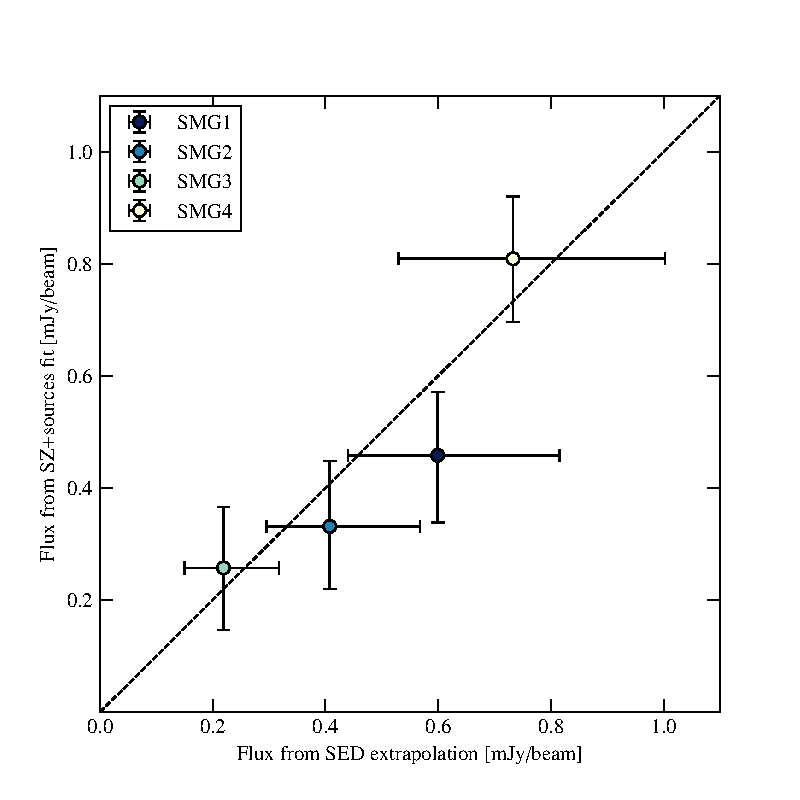
\includegraphics[width=0.5\linewidth, trim={.35cm .5cm .35cm 1.4cm}, clip]{Figures/Chap_actj0215/ps_fluxes_comp.pdf}
    \caption{%
        Comparaison des densités de flux des sources ponctuelles estimées par extrapolation de SED (abscisse) et par l'analyse jointe SZ--sources ponctuelles avec un \prior\ uniforme sur les flux (ordonnée, voir section \ref{sec:act:ps_flat_prior}).
        Les barres d'erreur représentent les 16èmes et 84èmes percentiles des distributions.
        Les deux estimateurs sont compatibles dans ces barres d'erreur pour chacune des sources.
    }
    \label{fig:act:pscomp}
\end{figure}


% ==================================================================================== %
\section{Résultats}

L'échantillonnage par MCMC décrit dans la section précédente est utilisé pour déterminer le jeu de paramètres $\vartheta$ qui ajuste le mieux la carte NIKA2 à 150 GHz.
Les modèles de carte de l'effet SZ, de contamination par les sources ponctuelles, et de la somme des deux contributions sont représentés dans la figure \ref{fig:act:dmr}.
Puisqu'aucune structure de rapport signal sur bruit significative n'est détectée dans les résidus, il est possible d'affirmer qu'il n'y a pas de signe de sous-structures ou d'asphéricité dans la carte NIKA2 de cet amas.

\begin{figure}[t]
    \begin{center}
    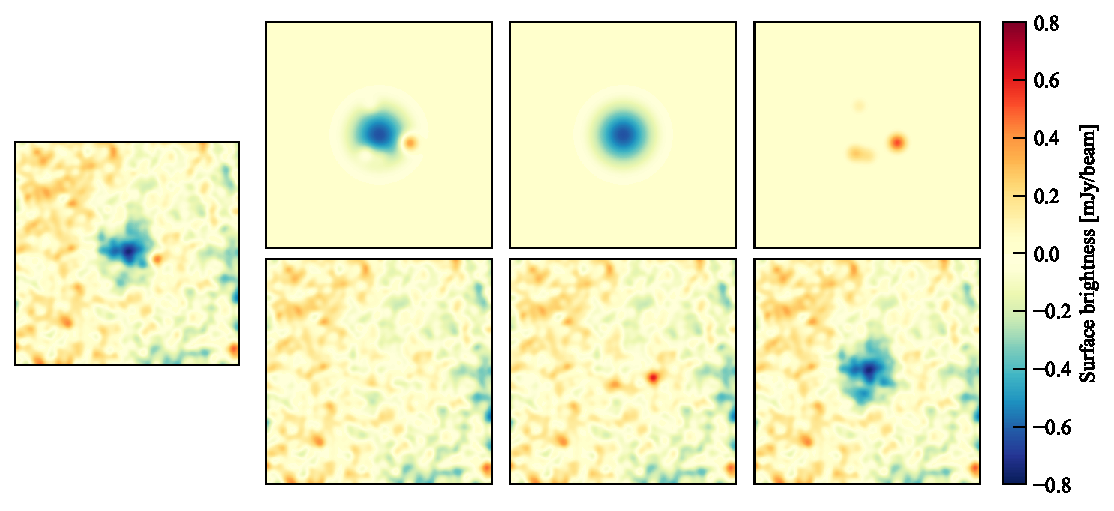
\includegraphics[width=.95\linewidth]{Figures/Chap_actj0215/dat_mod_res_full.pdf}
    \caption{%
        Résultats de l'ajustement de la carte NIKA2 à 150 GHz de \act\ (panneau de gauche).
        Le modèle ajustant le mieux les données et les résidus sont respectivement montrés dans les panneaux haut et bas de la colonne du centre gauche.
        Les colonnes de centre droit et droite représentent le meilleur modèle et les résidus en considérant seulement le signal SZ et les sources ponctuelles, respectivement.
        Les cartes sont représentées dans la même région et lissées par le même filtre que dans la figure \ref{fig:act:nkmaps}.
        Les deux sources dans le sud de la carte (S5 et S6) ont été soustraites.
        }
        \label{fig:act:dmr}
    \end{center}
\end{figure}

% ------------------------------------------------------------------------------------ %
\subsection{Thermodynamique du milieu intra-amas}

\begin{figure}[t]
    \centering
    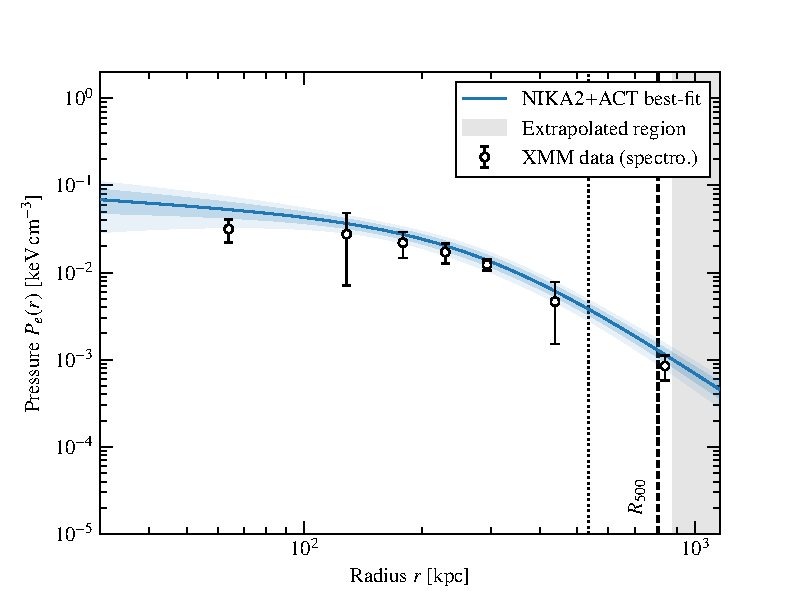
\includegraphics[page=1, width=.485\linewidth, trim={.3cm .1cm .9cm .8cm}, clip]{Figures/Chap_actj0215/ICM_thermodynamics.pdf}
    \includegraphics[page=2, width=.485\linewidth, trim={.3cm .1cm .9cm .8cm}, clip]{Figures/Chap_actj0215/ICM_thermodynamics.pdf}
    \includegraphics[page=3, width=.485\linewidth, trim={.3cm .1cm .9cm .8cm}, clip]{Figures/Chap_actj0215/ICM_thermodynamics.pdf}
    \includegraphics[page=4, width=.485\linewidth, trim={.3cm .1cm .9cm .8cm}, clip]{Figures/Chap_actj0215/ICM_thermodynamics.pdf}
    \caption{
        Profils radiaux de la pression (\textit{haut gauche}), température (\textit{haut droit}), entropie (\textit{cas gauche}), et masse hydrostatique (\textit{bas droit}) du milieu intra-amas de \act.
        Pour le profil de pression, la courbe bleue représente le profil de pression correspondant au meilleur ajustement des données NIKA2.
        Pour les autres profils, elle montre la combinaison entre ce profil de pression et le profil de densité obtenue avec \textit{XMM-Newton}.
        Les enveloppes bleues montrent les intervalles de confiance à $1\sigma$ et $2\sigma$ sur ces profils.
        Les points blancs représentent les profils obtenus en combinant les profils de densité et de température mesurés en X, avec des erreurs à $1\sigma$.
        La ligne noire en pointillés montre la limite à l'intérieur de laquelle le rapport signal sur bruit sur le profil de brillance de surface de la carte NIKA2 à 150 GHz est supérieur à $3\sigma$.
        La zone grisée représente la région dans laquelle les profils ne sont pas contraints par les données SZ, c'est-à-dire au delà de $R_{500}^\mathrm{ACT}$.
        }
        \label{fig:act:profiles}
\end{figure}

Le profil de pression obtenu à l'issue de l'analyse MCMC est présenté en haut à gauche de la figure \ref{fig:act:profiles}.
La ligne bleue correspond au maximum de vraisemblance de l'ajustement.
Les enveloppes d'erreur sont obtenues en calculant un profil de pression pour chaque jeu de paramètres échantillonné par le MCMC, puis la dispersion de ces profils en fonction de la distance au centre.
%
Ce profil est comparé à celui obtenu par combinaison des profils de densité et de température obtenus en X (représenté en blanc dans la figure \ref{fig:act:profiles}).
Cette comparaison est intéressante car les deux profils représentent deux mesures indépendantes de la distribution de pression dans le milieu intra-amas d'un amas distant et peu massif.
Les deux mesures sont en accord ; le profil de pression obtenu en SZ semble marginalement plus élevé, mais cet effet n'est pas significatif au vu des incertitudes sur les deux profils.

Plusieurs autres propriétés thermodynamiques peuvent être obtenues en combinant le profil de pression obtenu en SZ avec le profil de densité obtenu en X : le profil de température $T_\e(r)$, d'entropie $K_\e(r),$ et de masse hydrostatique $M_\mathrm{HSE}(<r)$ sont obtenus grâce à :
\begin{equation}
    k_\textsc{b} T_\e(r) = P_\e(r) \,\big/\, n_\e(r), \qquad K_\e(r) = P_\e(r)\;n_\e^{-5/3}(r),
\end{equation}
et à l'équation de l'équilibre hydrostatique :
\begin{equation}
    M_\mathrm{HSE}(<r) = -\frac{1}{\mu m_p G}\frac{r^2}{n_\e(r)}\frac{\d P_\e}{\d r},
    \label{eq:act:mhse}
\end{equation}
où $m_p$ est la masse du proton, $\mu$ le poids moléculaire moyen du gaz, et $G$ la constante de gravitation.
Ces profils sont présentés sur la figure \ref{fig:act:profiles}, en bleu tels qu'obtenus par combinaison de la densité X et de la pression SZ, et en blanc par combinaison de la densité et de la température X.
Comme pour la pression, les profils sont en accord, illustrant la complémentarité entre observations SZ à haute résolution et X.
Bien que cet amas ait bénéficié de temps d'observation similaires avec NIKA2 et \textit{XMM-Newton}, cette compatibilité illustre la grande qualité des mesures pouvant être obtenue en combinant les deux longueurs d'onde, minimisant la dépendance en observations de spectroscopie X pour la caractérisation des propriétés thermodynamiques du milieu intra-amas.
Enfin, cette combinaison permet d'atteindre une plus grande résolution sur le profil de température du milieu intra-amas que ce qui peut être atteint en spectroscopie X.
La figure \ref{fig:act:profiles} montre que l'extrapolation de la pente interne du profil de pression obtenu en spectroscopie X donne une température de cœur bien plus faible que celle obtenue par combinaison X-SZ.
Les incertitudes sur le profil de température sont également plus faibles en moyenne pour le profil NIKA2+XMM.
Par conséquent, les profils de masse et d'entropie présentent également des incertitudes plus faibles en combinant les observations X et SZ qu'en utilisant la spectroscopie X, résultant en une mesure plus précise des propriétés thermodynamiques du milieu intra-amas.

Les propriétés thermodynamiques de \act\ fournissent des renseignements sur l'état dynamique de son milieu intra-amas.
Le profil de pression est très plat dans la partie centrale de l'amas, indiquant un cœur perturbé.
La figure \ref{fig:act:profiles} compare le profil de pression obtenu dans cette analyse avec les profils de pression moyens obtenus en X et à bas redshift pour les amas de l'échantillon REXCESS \cite{arnaud_universal_2010}.
Le profil de pression de \act\ est mal décrit par le profil de pression dit universel, particulièrement dans le cœur de l'amas.
En revanche, il est bien décrit par le profil moyen des amas de l'échantillon REXCESS possédant un cœur perturbé.
La valeur de l'entropie ($K_{\e,\mathrm{core}} \gtrsim 200\;\mathrm{keV\cdot cm^2}$) et de la densité électronique ($n_{\e,\mathrm{core}} \lesssim 10^{-2}\;\mathrm{cm^{-3}}$) indiquent également un amas au cœur perturbé \cite{hudson_what_2010}.
La figure \ref{fig:act:profiles} compare le profil de pression obtenu dans cette analyse avec les profils de pression moyens obtenus en X et à bas redshift pour les amas de l'échantillon REXCESS \cite{arnaud_universal_2010}.
Le profil de pression de \act\ est mal décrit par le profil de pression universel, particulièrement dans le cœur de l'amas.
En revanche, il est bien décrit par le profil moyen des amas perturbés de l'échantillon REXCESS.
Des conclusions similaires ont également été tirées par \myciteauthor{ricci_xxl_2020}, en utilisant NIKA2 et \textit{XMM-Newton} pour caractériser le milieu intra-amas d'un autre amas distant de faible masse.
Ces conclusions sont intéressantes dans le cadre de discussions sur l'évolution de la fraction d'amas à cœur perturbé avec le redshift (par exemple, \cite{mcdonald_remarkable_2017,ruppin_stability_2020}).

\begin{figure}[t]
    \centering
    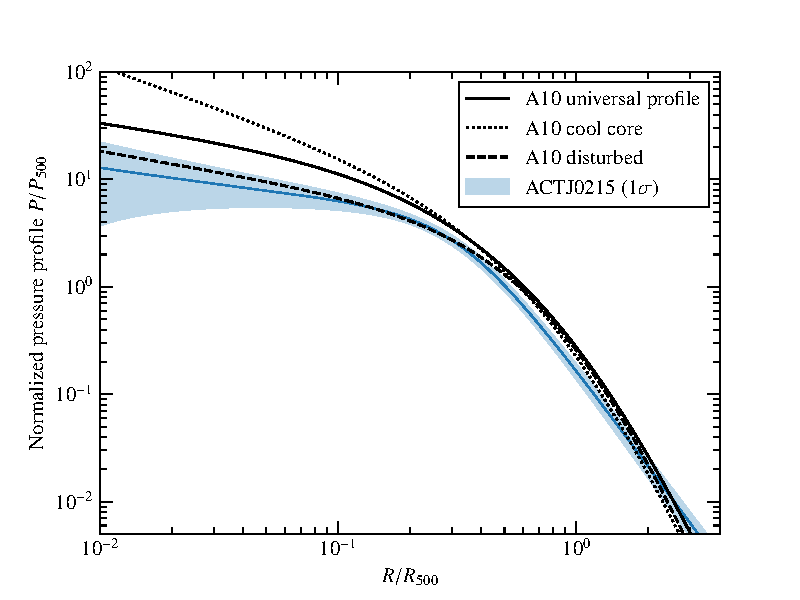
\includegraphics[width=0.6\linewidth, trim={.35cm .2cm .35cm 1cm}, clip]{Figures/Chap_actj0215/pressure_vs_upp.pdf}
    \caption{%
        Comparaison du profil de pression obtenu à partir des données NIKA2 (bleu) avec les profils moyens de \myciteauthor{arnaud_universal_2010} (noir).
        \act\ présente un profil similaire aux amas identifiés comme ayant un cœur perturbé (ligne noire pointillée).
        }
        \label{fig:act:press_upp}
\end{figure}

% ------------------------------------------------------------------------------------ %
\subsection{Grandeurs intégrées}

Pour des relevés SZ tels que ACT ou \textit{Planck}, la résolution angulaire ne permet pas de résoudre les amas distants, et la distribution radiale de leurs propriétés thermodynamiques ne peut donc pas être mesurée.
Par conséquent, les relations d'échelles utilisées pour calculer les masses des amas relient leur signal SZ intégré dans un rayon donné à la masse de l'amas contenue dans ce rayon.
Par exemple, le relevé ACT \cite{hasselfield_atacama_2013} utilise le rayon $R_{500}$, correspondant au rayon à l'intérieur duquel la densité moyenne est 500 fois supérieure à $\rho_c(z)$,la densité critique de l'Univers au redshift de l'amas.
Ce rayon peut être calculé comme le rayon pour lequel le contraste de densité $\delta_c$ vaut 500, c'est-à-dire en résolvant
\begin{equation}
    \delta_c(R_{500}) = \frac{M_\mathrm{HSE}(<R_{500})}{\rho_c(z) \times \frac{4}{3} \pi R_{500}^3} = 500.
\end{equation}
En utilisant le profil de masse hydrostatique obtenu par combinaison des profils X et SZ et présenté en figure \ref{fig:act:profiles}, on trouve
\begin{equation}
    R_{500} = 810.1 \pm 41.9 \, \mathrm{kpc},
\end{equation}
en accord avec la mesure du relevé ACT \cite{hasselfield_atacama_2013}.
Le paramètre de Compton intégré dans ce rayon peu alors être calculé :
\begin{equation}
    \mathcal{D}_\mathrm{A}^2 \; Y_{500} = (3.76 \pm 0.39)\times 10^{-5} \,\mathrm{Mpc^2},
\end{equation}
de même que la masse hydrostatique contenue dans le même rayon :
\begin{equation}
    M^\mathrm{HSE}_{500} = M_\mathrm{HSE}(<R_{500}) = (3.79 \pm 0.58) \times 10^{14} \,\mathrm{M}_\odot.
\end{equation}

Ces résultats sont présentés dans la table \ref{tab:act:integ}.
À des fins de comparaison, deux autres mesures de $R_{500}$ et $M_{500}$ y sont également rapportés, respectivement obtenus à partir de l'algorithme de détection d'amas dans le relevé ACT sous l'hypothèse d'un profil de pression universel, et à partir de l'analyse des seules données XMM-\textit{Newton} de \act.
L'incertitude sur la mesure de $Y_{500}$ est réduite d'un facteur 3 par rapport à la mesure du relevé ACT, indiquant un gain significatif en précision grâce aux observations SZ à haute résolution.
La valeur de $M_{500}$ obtenue à partir du profil de masse hydrostatique est compatible avec celle publiée dans le catalogue ACT, calculée avec la relation d'échelle $Y_{500}-M_{500}$ de \cite{arnaud_universal_2010}.
L'incertitude sur la masse est également plus faible dans cette étude que celle estimée dans le catalogue ACT, alors même que cette dernière est sous-estimée puisqu'elle ne tient pas compte de l'incertitude sur la relation d'échelle utilisée pour l'estimation (voir table~8 de \cite{hasselfield_atacama_2013}).
La valeur de masse obtenue par combinaison X-SZ est également compatible avec celle obtenue à partir de l'analyse X seule, bien que cette dernière soit plus faible en conséquence d'un rayon $R_{500}$ plus faible, et plus précise.

\begin{table}[t]
    \centering
    \small
    \begin{tabular}{c c c c}
        \toprule
        &  ACT  &  XMM-\textit{Newton}  &  NIKA2+XMM  \\
        \midrule
        \midrule
        $R_{500}$ & \multirow{2}{*}{$877.8 \pm 46.2$} & \multirow{2}{*}{$780.9 \pm 19.8$} & \multirow{2}{*}{$810.1 \pm 41.9$}  \\
        $[\mathrm{kpc}]$ &  &  &  \\
        \midrule
        $\mathcal{D}_\mathrm{A}^2 \; Y_{500}$ & \multirow{2}{*}{$4.07 \pm 1.13$} & \multirow{2}{*}{--} & \multirow{2}{*}{$3.76 \pm 0.39$} \\
        $\big[10^{-5}\;\mathrm{Mpc}^2\big]$ &  &  &  \\
        \midrule
        $M_{500}$ & \multirow{2}{*}{$3.5 \pm 0.8$} & \multirow{2}{*}{$2.48 \pm 0.70$} & \multirow{2}{*}{$3.79 \pm 0.58$}  \\[3pt]
        $\big[10^{14}\;\mathrm{M}_\odot\big]$ &  &  &  \\
        \bottomrule
    \end{tabular}
    \hspace{20pt}
    \caption{%
        Grandeurs intégrées caractéristiques de \act\ obtenue avec l'analyse des données ACT, \textit{XMM-Newton}, et NIKA2+\textit{XMM-Newton}.
        Les valeurs correspondant à l'analyse ACT proviennent de la table 8 de \cite{hasselfield_atacama_2013}.
    }
    \label{tab:act:integ}
\end{table}

% ==================================================================================== %
\section{Conclusions}

Le travail présenté dans ce chapitre constitue la première analyse individuelle d'un amas de galaxies du grand programme SZ de NIKA2 en utilisant des données de qualité standard.
Cette analyse a soulevé plusieurs difficultés.
Tout d'abord, l'amas analysé, \act, est un amas de basse masse et haut redshift dans l'échantillon du LPSZ, et de ce fait une source faible et compacte.
De plus, l'amas a été observé dans des conditions estimées suffisantes pour atteindre un rapport signal sur bruit de $3\sigma$ à $R_{500}$ sur le profil de brillance de surface SZ, objectif qui n'est pas atteint puisque le signal sur bruit ne vaut $3\sigma$ que jusqu'à $0.7 \times R_{500}$.
Enfin, le signal SZ détecté dans NIKA2 est fortement affecté par la présence de sources ponctuelles.
Cette contamination est particulièrement importante dans le cas de cet amas à cause du flux élevé des sources par rapport à celui de l'amas, mais également de sa faible extension spatiale.

En dépit de ces difficultés, de fortes contraintes ont pu être posées sur les propriétés thermodynamiques du milieu intra-amas de \act.
La contamination par les sources ponctuelles a été prise en compte dans une approche multifréquence basée sur une analyse jointe du signal SZ et des sources, permettant une propagation de l'incertitude sur l'amplitude de cette contamination aux résultats finaux.
Cette analyse a permis de mesurer la distribution radiale de pression du milieu intra-amas de l'amas, et de combiner ce résultat avec des mesures X pour caractériser plus largement la thermodynamique du milieu intra-amas de \act.

\vspace{5pt}
Les conclusions tirées de ces résultats sont les suivantes:
\begin{itemize}[leftmargin=*]
\setlength\itemsep{5pt}
\item
    Le profil de pression de \act\ est incompatible avec le profil de pression dit universel des amas de galaxies publié par \myciteauthor{arnaud_universal_2010}, mais en accord avec le profil des amas perturbés rapporté dans la même publication.
    Cela indique un cœur d'amas perturbé, en accord avec les autres propriétés thermodynamiques obtenues par combinaison avec des mesures X (telles que l'entropie au cœur de l'amas).

\item
    Les propriétés thermodynamiques obtenues en combinant les mesures NIKA2 et \textit{XMM-Newton} sans spectroscopie sont compétitives avec celles obtenues en utilisant des mesures X seules.
    Puisque les temps d'observation nécessaires à l'extraction d'information spectroscopique en X sont largement supérieurs à ceux nécessaires à l'obtention d'un profil de densité, et puisque ces temps augmentent rapidement avec le redshift, la combinaison d'observations SZ à haute résolution et X peu profondes apparaît comme un outil idéal pour la caractérisation du milieu intra-amas d'amas distants.

\item
    Les observations NIKA2 de cet amas ont permis d'améliorer la précision des mesures des profils thermodynamiques, de la masse et du signal SZ intégré de \act, à la fois par rapport au relevé ACT et à l'analyse X seule.
\end{itemize}

Cette analyse étant focalisée sur l'un des amas les plus complexes du LPSZ, il est raisonnable d'attendre de telles conclusions pour la plupart des analyses individuelles de l'échantillon.
Ces résultats sont donc très prometteurs pour l'étude du profil de pression moyen et de la relation d'échelle $Y_{500}-M_{500}$ grâce au LPSZ.
